\input{"preamble.tex"}


\let\Begin\begin
\let\End\end
\newcommand\wrapenv[1]{#1}

\makeatletter
\def\ScaleWidthIfNeeded{%
 \ifdim\Gin@nat@width>\linewidth
    \linewidth
  \else
    \Gin@nat@width
  \fi
}
\def\ScaleHeightIfNeeded{%
  \ifdim\Gin@nat@height>0.9\textheight
    0.9\textheight
  \else
    \Gin@nat@width
  \fi
}
\makeatother

\setkeys{Gin}{width=\ScaleWidthIfNeeded,height=\ScaleHeightIfNeeded,keepaspectratio}%

\title{
\textbf{
    Title
  }
  }







\begin{document}

\date{}
\author{D. Zack Garza}
\maketitle


\newpage

% Note: addsec only in KomaScript
\addsec{Table of Contents}
\tableofcontents
\newpage

\hypertarget{saturday-june-05-perspectives-on-nonabelian-hodge-theory}{%
\section{Saturday, June 05: Perspectives on nonabelian Hodge
theory}\label{saturday-june-05-perspectives-on-nonabelian-hodge-theory}}

\begin{remark}

Abstract: The nonabelian Hodge correspondence provides a rich interplay
of structures from topology, analysis and algebraic geometry which has
spurred the curiosities of specialists and non-specialists alike. In the
first part of this talk I will outline the celebrated nonabelian Hodge
correspondence, due to Carlos Simpson, identifying certain
representations of the fundamental group of a smooth projective complex
variety with semistable ``Higgs'' bundles. I will discuss the
consequences of this identification at the level of moduli spaces
parametrizing these objects. Time permitting, I will survey more recent
extensions to the characteristic p or p-adic settings.

I will begin the second half of the lecture with a discussion of the
Hodge filtration on nonabelian cohomology. Understanding the framework
of filtrations set forth allows for us to view the nonabelian Hodge
correspondence in a general light. Indeed, it becomes a manifestation of
the following general question: when is a graded object canonically the
associated graded of a filtered object? I will conclude this talk with a
discussion of some work of mine bringing this perspective into the
setting of higher algebra and higher categories, along with joint work
with Robalo and Toën applying this perspective towards an understanding
of the HKR filtration on Hochschild homology.

\end{remark}

\hypertarget{part-1}{%
\subsection{Part 1}\label{part-1}}

\begin{quote}
Tasos Mouliunos: Perspectives on Nonabelian Hodge Theory (Talbot 2011)
\end{quote}

For \((X, g)\) a Riemannian manifold, construct the de Rham complex
\(\omega^*_X = C^\infty(X) \mapsvia{d} \Omega^1_X \mapsvia{d} \cdots\).
Using a metric we can define an adjoint operator
\(\delta: \Omega^* \to \Omega^*[-1]\). Defining the Laplacian as
\(\laplacian \da \delta d + d\delta\), and a differential \(n\dash\)form
is harmonic of \(\laplacian \omega= 0\). Recall that Hodge theorem:
there is an isomorphism

??

So there are harmonic representatives for de Rham cohomology classes.

Assume \(X\) is a smooth projective complex variety, or more generally a
Kähler. There is a decomposition
\(\Omega_X^n \tensor_\RR \CC = \bigoplus _{p+q=n} \Omega^{p, q}_X\)
which is \(p\) exterior powers of \(\Omega^{1, 0}\) wedge with \(q\)
exterior powers of \(\Omega^{0, 1}\). There is also a decomposition
\(d = \del + \delbar\) with \(\del\) raises degree \(p\) by 1 and
\(\delbar\) raises degree \(q\) by 1. There are formal adjoints to
\(\del, \delbar\), and one defines
\(\laplacian_d, \laplacian_{\del}, \laplacian_{\delbar}\) analogously.
There are Kahler identities:
\begin{align*}
\laplacian_d = 2 \laplacian_{\del} = 2\laplacian_{\delbar}
.\end{align*}

\begin{quote}
Todo: check
\end{quote}

\begin{theorem}[?]

There is a decomposition
\begin{align*}
H^n(X; \CC) \cong \bigoplus _{p+q = n} H^{p, q}(X)
.\end{align*}
where
\begin{align*}
H^{p, q} = D^p_{\Dolbeaut}(X; \Omega_X^q) = \mathcal{H}^{p, q}(X)
,\end{align*}
and the latter is the vector space of harmonic forms of degree \(p, q\).

\end{theorem}

\begin{remark}

This data yields a finite decreasining filtration \(F\) together with a
conjugate filtration \(\bar F\) on \(H^{p, q}\) where
\(F_p(H) \intersect \bar{F}_p(H) = H^n\) and yields a notion of
\emph{pure Hodge structure of weight \(n\)}.

\end{remark}

\begin{remark}

By GAGA, there is a correspondence between holomorphic and complex
algebro-geometric data for nice enough sheaves. This mixes

\begin{itemize}
\tightlist
\item
  Topological data: \(H^n(X; \CC)\)
\item
  Smooth data: \(H^n_{\dR}(X)\)
\item
  Holomorphic/complex algebro-geometric data: the decomposition into
  harmonic forms.
\end{itemize}

Nonabelian Hodge theory is an attempt to categorify this fact.

\end{remark}

\begin{theorem}[?]

There is an equivalence of categories
\begin{align*}
\correspond{
  \text{Local systems of } \Vect_\CC \\ \text{on }X
}
&\mapstofrom
\correspond{
  \text{Complex vector bundles on } X \\ \text{with a flat connection}
}
\end{align*}

\end{theorem}

\begin{remark}

The right-hand side can be identified with monodromy representations
\(\rho: \pi_1(X) \to \GL_n(\CC)\).

\begin{quote}
Missed some stuff.
\end{quote}

We'll want \(H^1(X; \GL_n(\CC))\) to be the space of such
representations. How do we make sense of the Hodge decomposition here?
The answer: a vector bundle with a Higgs field, i.e.~a Higgs bundle: a
pair \((E, \theta)\) where \(E\) is a complex bundle. There are also
\emph{harmonic bundles} which interpolates between Higgs bundles and
flat bundles. Harmonic bundles: bundle with \(\del, \delhar\) with
algebraic operators
\(\theta, \bar\theta \in \Gamma(X, \Endo(E) \tensor \Omega^1)\). One can
fix a Hermitian metric so that \(\del + \delbar\) is a unitary
connection and \(\theta + \bar\theta\) is self-adjoint.

\end{remark}

\begin{remark}

\(\delbar\) defines a holomorphic structure on \(E\) by the
Koszul-Malgrange theorem, yielding a holomorphic bundle. Given a bundle
with flat connection and a Hermitian metric, one can define the data
\(D_K''\) needed for a Higgs structure, but then one needs to solve the
system of PDEs \((D_K'')^2=0\). Conversely, given a Higgs bundle \(E\),
namely \(\theta'' = \theta + \delbar\), one can define a connection
\(D_K\) and if \((D_K)^2=0\) then this is a flat connection.

\end{remark}

\begin{theorem}[Nonabelian Hodge theorem]

Let \(X\) be a smooth complex projective variety.

\begin{itemize}
\tightlist
\item
  There is an equivalence of categories: harmonic bundles on \(X\) and
  semisimple flat bundles (or equivalently \(\pi_1(X)\) representations)
\item
  There is an equivalence of categories: harmonic bundles and direct
  sums of stable Higgs bundles with vanishing Chern classes
  \(c_1(E) = c_2(E) = 0\).
\end{itemize}

\begin{quote}
Something else?
\end{quote}

\end{theorem}

\begin{remark}

Semi-stability is a condition on coherent subsheaves.

\end{remark}

\begin{remark}

Consider the degree 1 case of the Hodge correspondence.
\(H^1(X; \GL_n(\CC))\) should be a moduli stack. LEt
\(F: \CAlg_k^0 \to \Gpd\) be a functor, then it's representable by a
stack, which is typically required to satisfy descent with respect to a
topology on \(\CAlg_k\) (a gluing condition, e.g.~etale descent). Can
realize quotient stacks as a simplicial object in groupoids? Can also
take GIT quotients, \(\spec R^G\) of the invariants.

\end{remark}

\begin{remark}

Use the functor of points to define the Betti moduli space. Higgs moduli
space: semistable Higgs bundles with vanishing Chern classes and a frame
at \(x\), i.e.~\(E \cong \CC^n\).

\end{remark}

\begin{remark}

There is an equivalence between \(R_\dR\) and \(R_B\), the de Rham and
Betti moduli stacks? Can get an equivalence of categories without
underling topological spaces being homeomorphic?

\end{remark}

\begin{remark}

Semisimple flat bundles fixed by a \(\GG_m\) action are those which
underlie complex variations of Hodge structure. These show up in
relative de Rham cohomology. See Riemann-Hilbert correspondence?

\end{remark}

\hypertarget{part-2}{%
\subsection{Part 2}\label{part-2}}

\begin{remark}

We want to consider an analog of the Hodge filtration for nonabelian
cohomology. In the classical case, Hodge decompositions correspond to
descreasing filtrations on \(H^*(X; \CC)\). Think of
\(H^1(X, \GL_n(\CC))\) as a complex linear mapping stack
\(\mcm_B(X, n) \da \Map(\pi_1(X), \GL_n) / \GL\), we'll want a
filtration on this.

\end{remark}

\begin{remark}

Recalling the Rees construction, we have
\begin{align*}
F^*(V) = \qty{\cdots \to F^{p+1} V \to F^p V \to \cdots } && V\da \colim F^*(V) 
.\end{align*}
We'll map \(F^*(V)\) to \(\xi(V, F)\), which will be a submodule of
\(V \tensor \CC[t, t\inv]\) generated by \(t^{-p} F^p(V)\), which is
like a \(\CC[t]\dash\)lattice in \(V\tensor \CC[t, t\inv]\) and thus a
module over \(\CC[t]\). Equip it with a Galois action to get a free
sheaf over \(\AA^1 = \spec \CC[t]\) with a \(\GG_m\dash\)action.

\end{remark}

\begin{remark}

Upshot: we'll get an equivalence of categories between
\(\GG_m\dash\)equivariant vector bundles over \(\AA^1\) with filtered
vector spaces. We realize \(\AA_1/\GG_m\) as the realization of a
simplicial object:
\begin{align*}
\AA_1/\GG_m = \realize{ \AA^1 \simplicialone A^1 \cross \GG_m \simplicialtwo \cdots }
.\end{align*}

\end{remark}

\begin{remark}

Diagram:

\begin{figure}
\centering
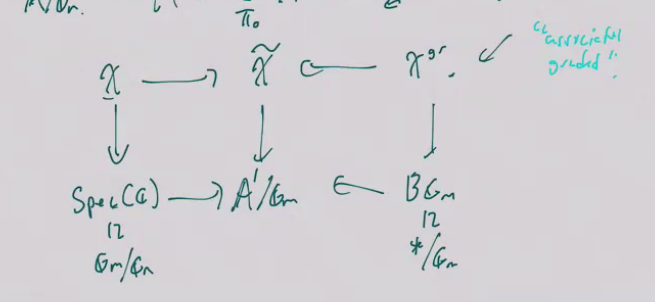
\includegraphics{figures/image_2021-06-05-16-13-37.png}
\caption{These are pullback squares}
\end{figure}

This endows \(R \gamma(X, \OO_X)\) with a filtration

\end{remark}

\hypertarget{hodge-filtration-on-nonabelian-cohomology}{%
\subsubsection{Hodge Filtration on Nonabelian
Cohomology}\label{hodge-filtration-on-nonabelian-cohomology}}

\begin{remark}

We realize \(H^1(X, \GL_n(\CC))\) as a stack and take the de Rham stack
\(\mcm_{\dR}(X, n)\) over \(\spec \CC\). A filtration will be an
\(\tilde \mcm\) fitting into a pullback:

\begin{figure}
\centering
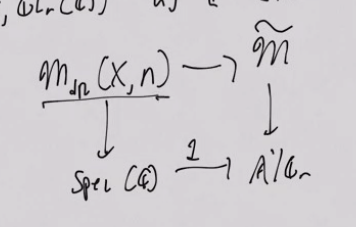
\includegraphics{figures/image_2021-06-05-16-15-27.png}
\caption{image\_2021-06-05-16-15-27}
\end{figure}

Similarly, to obtain \(\mcm_{\Dolbeaut}\) (the moduli stack of Higgs
bundles) as
\(\mcm_{\Dolbeaut}(X, n) \simeq \mcm \fiberprod_{\AA^1/\GG_m} \B \GG_m\).
The idea (going back to Deligne): construct a 1-parameter family.

\end{remark}

\begin{definition}[?]

Fix \(E\) a complex vector bundle, then a
\textbf{\(\lambda\dash\)connection} is an operator
\begin{align*}
\nabla_{\lambda}: E\to \E\tensor \Omega_X^1
&&
\nabla_{\lambda}(rf) = \lambda d(r) f + r\nabla(f), \nabla_{\lambda}^2 = 0
\end{align*}
where \(r\) is a coefficient and \(f\) is a section of \(E\) and \(d\)
is the de Rham differential.

\end{definition}

\begin{remark}

If \(\lambda=0\) this reduces to \(\nablda(rf) = r\nabla(f)\). Setting
\(\theta \da \nabla_0\) yields precisely the data of the Higgs field.
For \(\lambda=1\) this recovers the notion of a flat connection.

\end{remark}

\begin{proposition}[Key]

A harmonic bundle \((E, D, D'')\), where \(D, D''\) are operators, gives
rise to a family of flat \(\lambda\dash\)connections with

\begin{itemize}
\tightlist
\item
  A flat part \((E_1, D_1) = (E, 0)\)?
\item
  A Higgs part \((E_0, \nabla_0) = (E,\ theta)\)
\end{itemize}

\end{proposition}

\begin{theorem}[Simpson]

Let \(S\) be a scheme over \(\AA^1\), then there is a functor
\begin{align*}
(\lambda:S\to \AA^1) \to (E, \nabla, \alpha)
\end{align*}
where - \(E\) is a bundle over \(X\cross S\), - \(\nabla\) is a
\(\lambda\dash\)connection, and - \(\alpha: E \ro{x} \cong \CC^n\) is a
frame

is representable by \(R^{\Hodge}(X, n) \to \AA^1\) which yields a map
\begin{align*}
\mcm^{\Hodge}(X, n) / \GL_n \to \AA^1
.\end{align*}
Setting \(\mcm \da \mcm^\Hodge(X, n)\), \(\mcm\) admits a \(\CC^*\)
action and since \(\CC^* \cong \GG_m\) we get
\begin{align*}
\mcm/\GG_m \to \AA^1/\GG_m
.\end{align*}
When \(\lambda\) is invertible we recover flat connections, and so there
is a pullback:

\begin{center}
\begin{tikzcd}
    {\mcm_\dR \cross \GG_m} && \mcm \\
    \\
    {\GG_m} && {\AA^1}
    \arrow[from=1-3, to=3-3]
    \arrow[from=3-1, to=3-3]
    \arrow[from=1-1, to=1-3]
    \arrow[from=1-1, to=3-1]
    \arrow["\lrcorner"{anchor=center, pos=0.125}, draw=none, from=1-1, to=3-3]
\end{tikzcd}
\end{center}

\begin{quote}
\href{https://q.uiver.app/?q=WzAsNCxbMCwwLCJcXG1jbV9cXGRSIFxcY3Jvc3MgXFxHR19tIl0sWzAsMiwiXFxHR19tIl0sWzIsMCwiXFxtY20iXSxbMiwyLCJcXEFBXjEiXSxbMiwzXSxbMSwzXSxbMCwyXSxbMCwxXSxbMCwzLCIiLDEseyJzdHlsZSI6eyJuYW1lIjoiY29ybmVyIn19XV0=}{Link
to Diagram}
\end{quote}

Using that \(\spec k \mapsvia{0} \AA^1\), pulling back recovers
\(\mcm^{\Hodge}\).

\end{theorem}

\begin{remark}

The conditions of semistability and vanishing Chern classes together
allow us to lift a category of objects with an intrinsic notion of
grading, e.g.~\(\mcm^\Dolbeaut \to \B \GG_m\), to a category with an
intrinsic notion of a filtration, e.g.~over \(\AA^1/\GG_m\).

\end{remark}

\hypertarget{higher-algebra}{%
\subsubsection{Higher Algebra}\label{higher-algebra}}

\begin{remark}

Given a stable infinity category \(\cat{C}\) we can make sense of
filtered objects in \(\cat{C}\), so filtered spectra make sense:
\begin{align*}
\Sp^{\fil}: E(1) \to E(0) \to E(-1) \to \cdots
.\end{align*}
By spectral algebraic geometry, affines are connective
\(E_\infty\dash\)rings. We have

\begin{itemize}
\tightlist
\item
  \(\spec \SS\)
\item
  \(\spec \SS[\NN] \cong \AA^1\)\footnote{Note that there are two
    notions of affine line here, but this is the more commonly used one.}
\item
  \(\spec \SS[\ZZ] = \GG_m\)
\end{itemize}

So we can define \(\AA^1/\GG_m\), and we can defined an infinity
category of quasicoherent sheaves

\begin{align*}
\Tot\qty{ \modsleft{\SS[\NN]} \simplicialone \modsleft{\SS[\NN \cross \ZZ]} \simplicialtwo \cdots } 
\simeq \QCoh(\AA^1/\GG_m)
.\end{align*}

\end{remark}

\begin{theorem}[?]

There is a symmetric monoidal equivalence of categories
\begin{align*}
\QCoh(\AA^1/\GG_m) \simseq \Sp^{\fil}
,\end{align*}
where the right-hand side is equipped with the Day convolution product.

\end{theorem}

\begin{remark}

Pulling back a qcoh sheave from \(\AA^1/\GG_m\) is taking a colimit of
underlying objects, whereas pulling back from \(\B \GG_m\) amounts to
taking the associated graded?

As a consequence, we can import nonabelian Hodge theory into the setting
of higher categories.

\end{remark}

\begin{question}

Suppose \(\cat{C}^0 \subseteq \cat{C}\) is a ``graded infinity
category'', when does \(\cat{C}^0\) lift to a category ??? over
\(\QCoh(\AA^1/\GG_m)\).

\end{question}

\begin{remark}

On Hochschild homology: there is the HKR filtration of \(\HH(R/k)\) we
have
\begin{align*}
\HH(R/k) &= S^1 \tensor_k R \\
\Spec (S^1 \tensor_k R) &= \Map(S^1, \Spec R)
\end{align*}
where the second line comes from derived geometry.

\end{remark}

\begin{theorem}[MRT]

Construct a stack \(S^1_\fil \to\AA^1/\GG_m\) and define a loop stack
\begin{align*}
\mcl_\fil(k) = \Map_{\AA^1/\GG_m} (S^1_\fil, X)
.\end{align*}

We get a diagram where the left recovers Hochschild homology and the
right recovers the de Rham algebra:

\begin{figure}
\centering
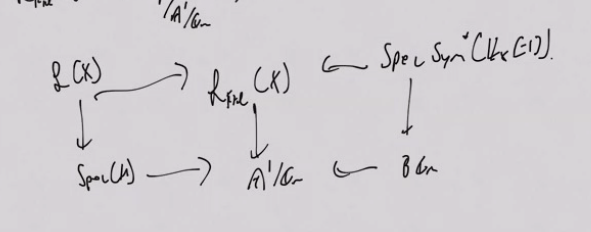
\includegraphics{figures/image_2021-06-05-16-40-51.png}
\caption{image\_2021-06-05-16-40-51}
\end{figure}

\end{theorem}

\begin{remark}

The top-right corner is a ``mixed complex''. Note that there is an
\(S^1\) action on \(\mcl(X)\) and an \(S^1_\fil\) action on
\(\mcl_\fil(X)\)? We have a lift of the mixed complex to a filtered
object whose underlying complex is HH?

\end{remark}

\begin{remark}

There is a map \(\mcl(X) \to \mcl_\Fil(X)\to \mcl_X[-1]\) which gives a
2-fold bar construction which relates to the degeneration of de Rham to
Dolbeault moduli spaces.

\end{remark}




\end{document}
